{

\pagestyle{fancy}

\pagestyle{fancy}
\fancyhead{}


\hypersetup{linkcolor=black}

\lhead{Table des matières}

% Table of contents -------------------------------------------------
\tableofcontents\thispagestyle{fancy}
\listoffigures
\listoftables

% Chapter 1 ---------------------------------------------------------
% -------------------------------------------------------------------
\pagebreak
\lhead{Introduction}
\chapter{Introduction}\thispagestyle{fancy}


\section{Présentation du projet}
It contains sophisticated software tools and components with which you can construct (typeset) a wide range of documents. The sub-title of this article also poses two questions about .

\subsection{Idée initiale}
h you can construct (typeset) a wide range of documents. The sub-title of this art

\subsection{Solution de la problematique}
h you can construct (typeset) a wide range of documents. The sub-title of this art


\section{Etat de l'art}

\subsection{Les services offertes}
h you can construct (typeset) a wide range of documents. The sub-title of this art

\subsection{Comparison avec autres produits}
h you can construct (typeset) a wide range of documents. The sub-title of this art



% Chapter 2 ---------------------------------------------------------
% -------------------------------------------------------------------

\pagebreak
\lhead{Version I}

\chapter{Version I}\thispagestyle{fancy}
\section{Raspberry PI}
In terms, “the new kid on the block” despite having been in active development for over 10 years.

\section{API}
In terms, “the new kid on the block” despite having been in active development for over 10 years.
\begin{center}

\begin{figure}[h]
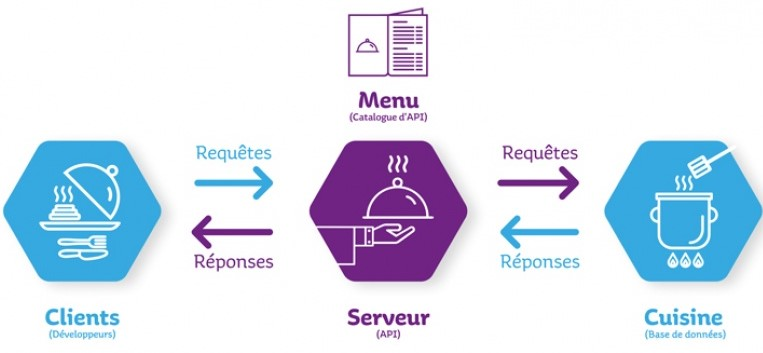
\includegraphics[width=18cm, height=9cm]{3-Figures/api.jpg}\\[2cm]
\caption{API}
\label{fig:figure2}
\end{figure}
\Large

\end{center}


\section{Modèles Deep learning}
In terms, “the new kid on the block” despite having been in active development for over 10 years.
\subsection{Facial recognition}
\subsubsection{Dataset}

\subsubsection{LBH}
development for over 10 years
\subsubsection{CNN}
development for over 10 years
\subsection{Tesseract OCR}
\subsection{YOLOv4}
Object detection is a computer technology related to computer vision and image processing that deals with detecting instances of semantic objects of a certain class (such as humans, buildings, or cars) in digital images and videos.[1] Well-researched domains of object detection include face detection and pedestrian detection. Object detection has applications in many areas of computer vision, including image retrieval and video surveillance.

Methods for object detection generally fall into either neural network-based or non-neural approaches. For non-neural approaches, it becomes necessary to first define features using one of the methods below, then using a technique such as support vector machine (SVM) to do the classification. On the other hand, neural techniques are able to do end-to-end object detection without specifically defining features, and are typically based on convolutional neural networks (CNN).

Non-neural approaches:
Viola–Jones object detection framework based on Haar features
Scale-invariant feature transform (SIFT)
Histogram of oriented gradients (HOG) features[6]
Neural network approaches:
Region Proposals (R-CNN,[7] Fast R-CNN,[8] Faster R-CNN,[9] cascade R-CNN.[10])
Single Shot MultiBox Detector (SSD) [11]
You Only Look Once (YOLO) [12][13][14][5][15]
Single-Shot Refinement Neural Network for Object Detection (RefineDet) [16]
Retina-Net [17][10]
Deformable convolutional networks [

% Chapter 3 ---------------------------------------------------------
% -------------------------------------------------------------------
\pagebreak

\lhead{Version II}
\chapter{Version II}\thispagestyle{fancy}
\section{Raspberry PI}
In terms, “the new kid on the block” despite having been in active development for over 10 years.

\section{Sockets}
In terms, “the new kid on the block” despite having been in active development for over 10 years.

\section{Modèles Deep learning}
In terms, “the new kid on the block” despite having been in active development for over 10 years.
\subsection{LBH}
\subsection{Handwritting recognition}
\subsection{YOLOv4 80 classes}


% Chapter 4 ---------------------------------------------------------
% -------------------------------------------------------------------

\pagebreak
\lhead{Démonstration}
\chapter{Démonstration}\thispagestyle{fancy}

% Chapter 5 ---------------------------------------------------------
% -------------------------------------------------------------------

\pagebreak
\lhead{Organisation}

\chapter{Organisation}\thispagestyle{fancy}
\section{Gantt}
A Gantt chart is a type of bar chart that illustrates a project schedule, named after its popularizer, Henry Gantt, who designed such a chart around the years 1910–1915. Modern Gantt charts also show the dependency relationships between activities and the current schedule status

\section{Github}
GitHub, Inc. is a provider of Internet hosting for software development and version control using Git. It offers the distributed version control and source code management functionality of Git, plus its own features

\section{Budget}
GitHub, Inc. is a provider of Internet hosting for software development and version control using Git. It offers the distributed version control and source code management functionality of Git, plus its own features

% Chapter 6 ---------------------------------------------------------
% -------------------------------------------------------------------


\pagebreak
\lhead{Code source du projet}
\chapter{Code source du projet}\thispagestyle{fancy}
Vous trouvez dans ce \href{https://github.com/mohammedAljadd/iEars}{lien} le code source de notre projet inclu les deux versions.\\

\begin{center}
\begin{figure}[h]
\centering
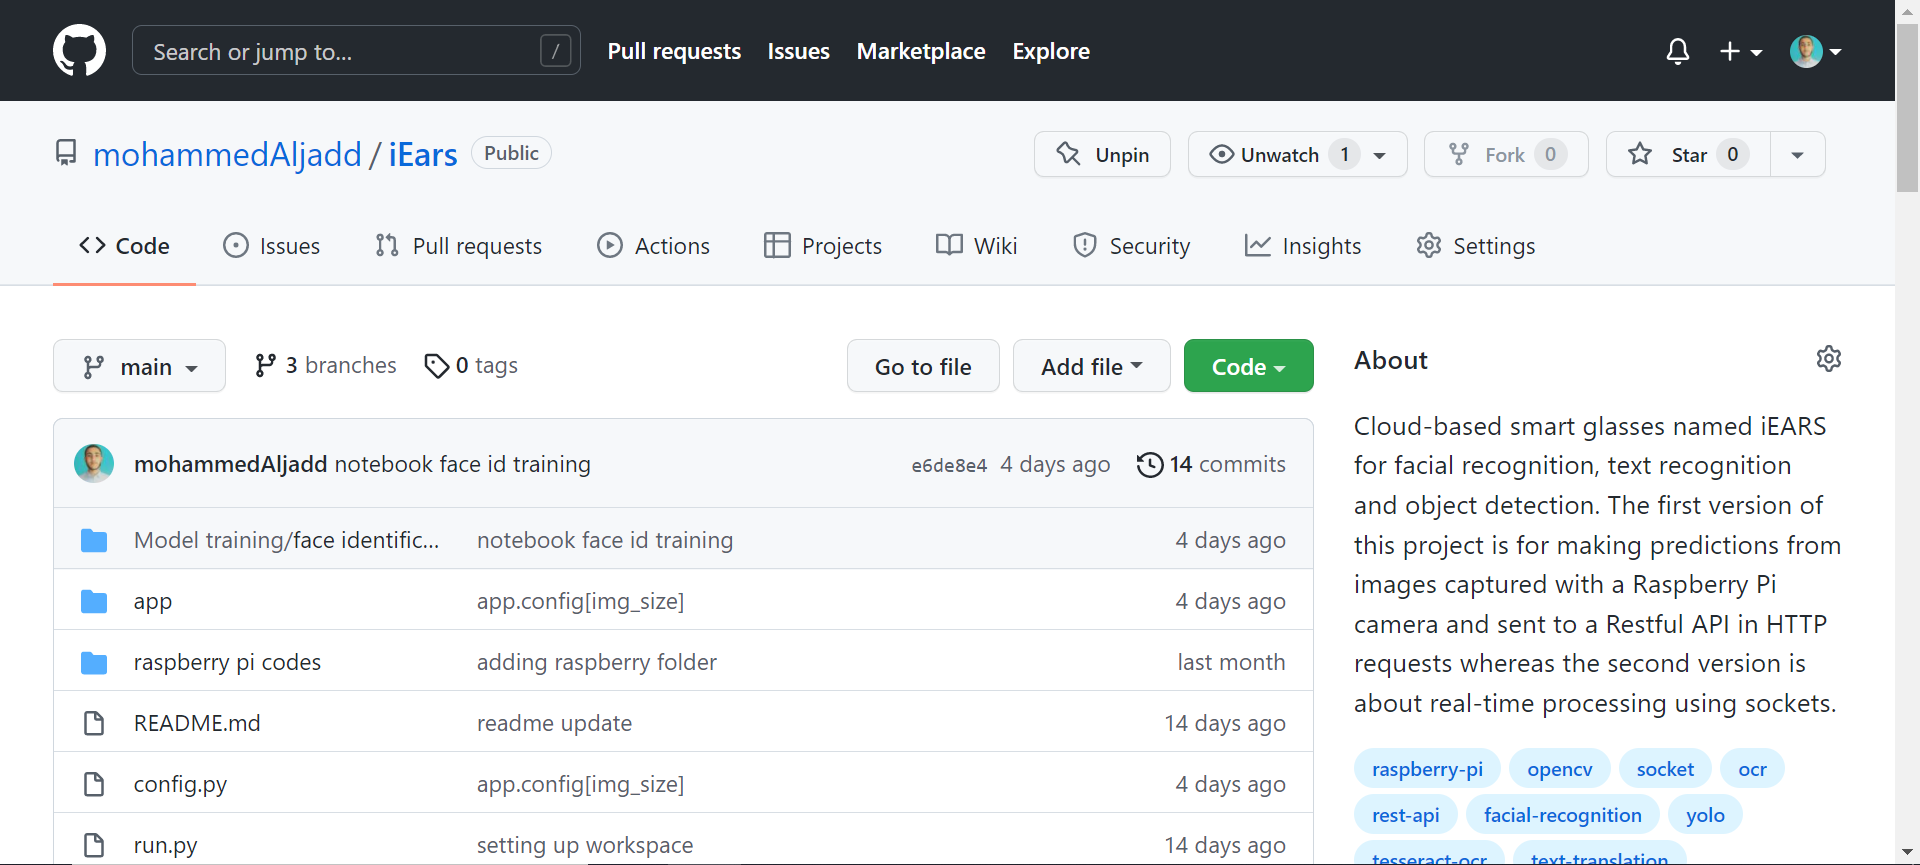
\includegraphics[width=18cm, height=9cm]{4-Images/github.PNG}\\[2cm]
\caption{Github}
\label{fig:figure2}
\end{figure}
\Large

\end{center}

% Chapter 7 ---------------------------------------------------------
% -------------------------------------------------------------------

\pagebreak
\lhead{Bibliographie}
\chapter*{Bibliographie}
\printbibliography 

}